\documentclass{gost}

%-------------------------------------------------------------------------------
%
% ПЕРЕМЕННЫЕ
%
%-------------------------------------------------------------------------------

\newcommand{\universityFullName}{Федеральное государственное бюджетное
образовательное учреждение высшего образования Саратовский Государственный
Технический Университет имени Гагарина Ю.А.}
\newcommand{\universityShortName}{СГТУ им. Гагарина Ю.А.}
\newcommand{\department}{Прикладные информационные технологии}
\newcommand{\nirName}{Лабораторная работа по основам работы с разделами жесткого
диска и файловой системой в ОС Unix}
\newcommand{\nirType}{промежуточный}
\newcommand{\nirStage}{1}
\newcommand{\subject}{Программные и аппаратные технологии умного города}

%-------------------------------------------------------------------------------
%
% ДОКУМЕНТ
%
%-------------------------------------------------------------------------------

\begin{document}
	\gostTitlePage

	\section{Создание виртуального жесткого диска}
		\begin{figure}[H]
			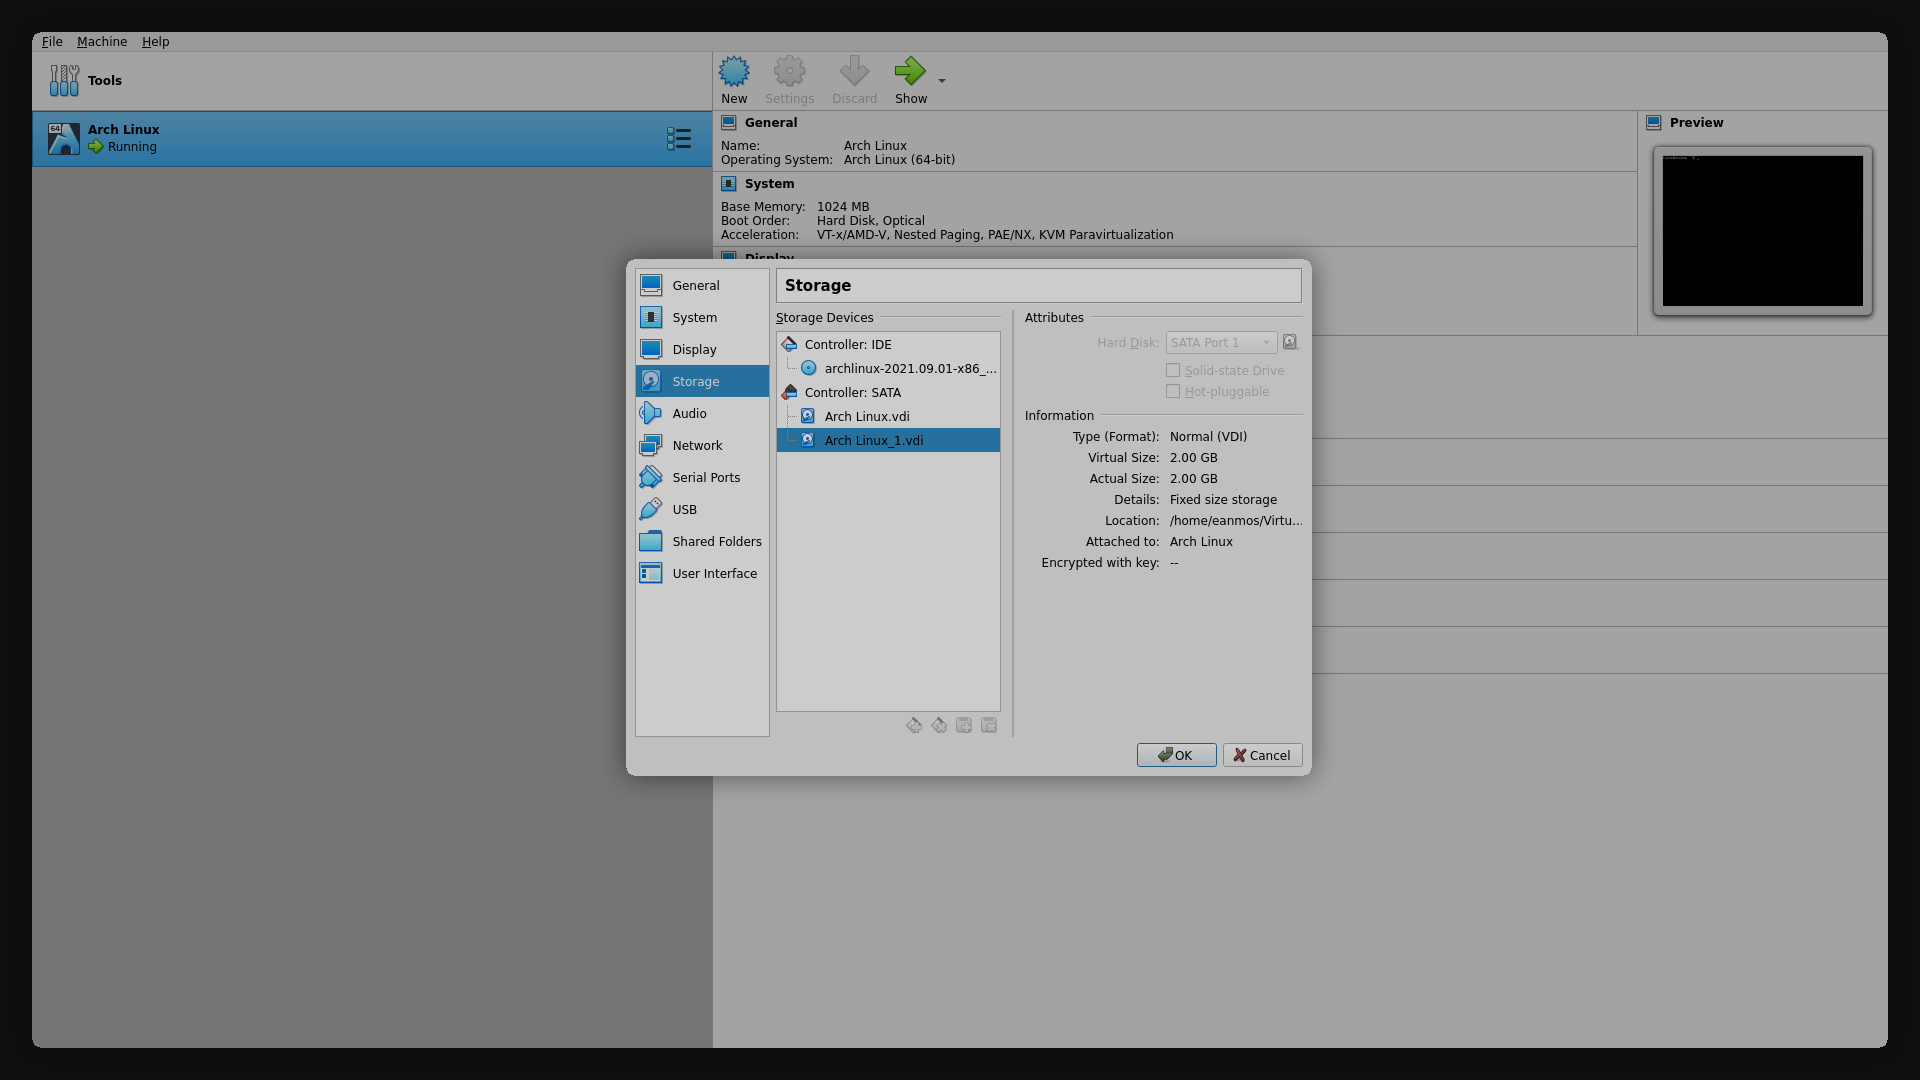
\includegraphics[width=\textwidth,clip=true]{img/1.png}
			\caption{Диалог создания виртуального жесткого диска}
		\end{figure}

		\begin{figure}[H]
			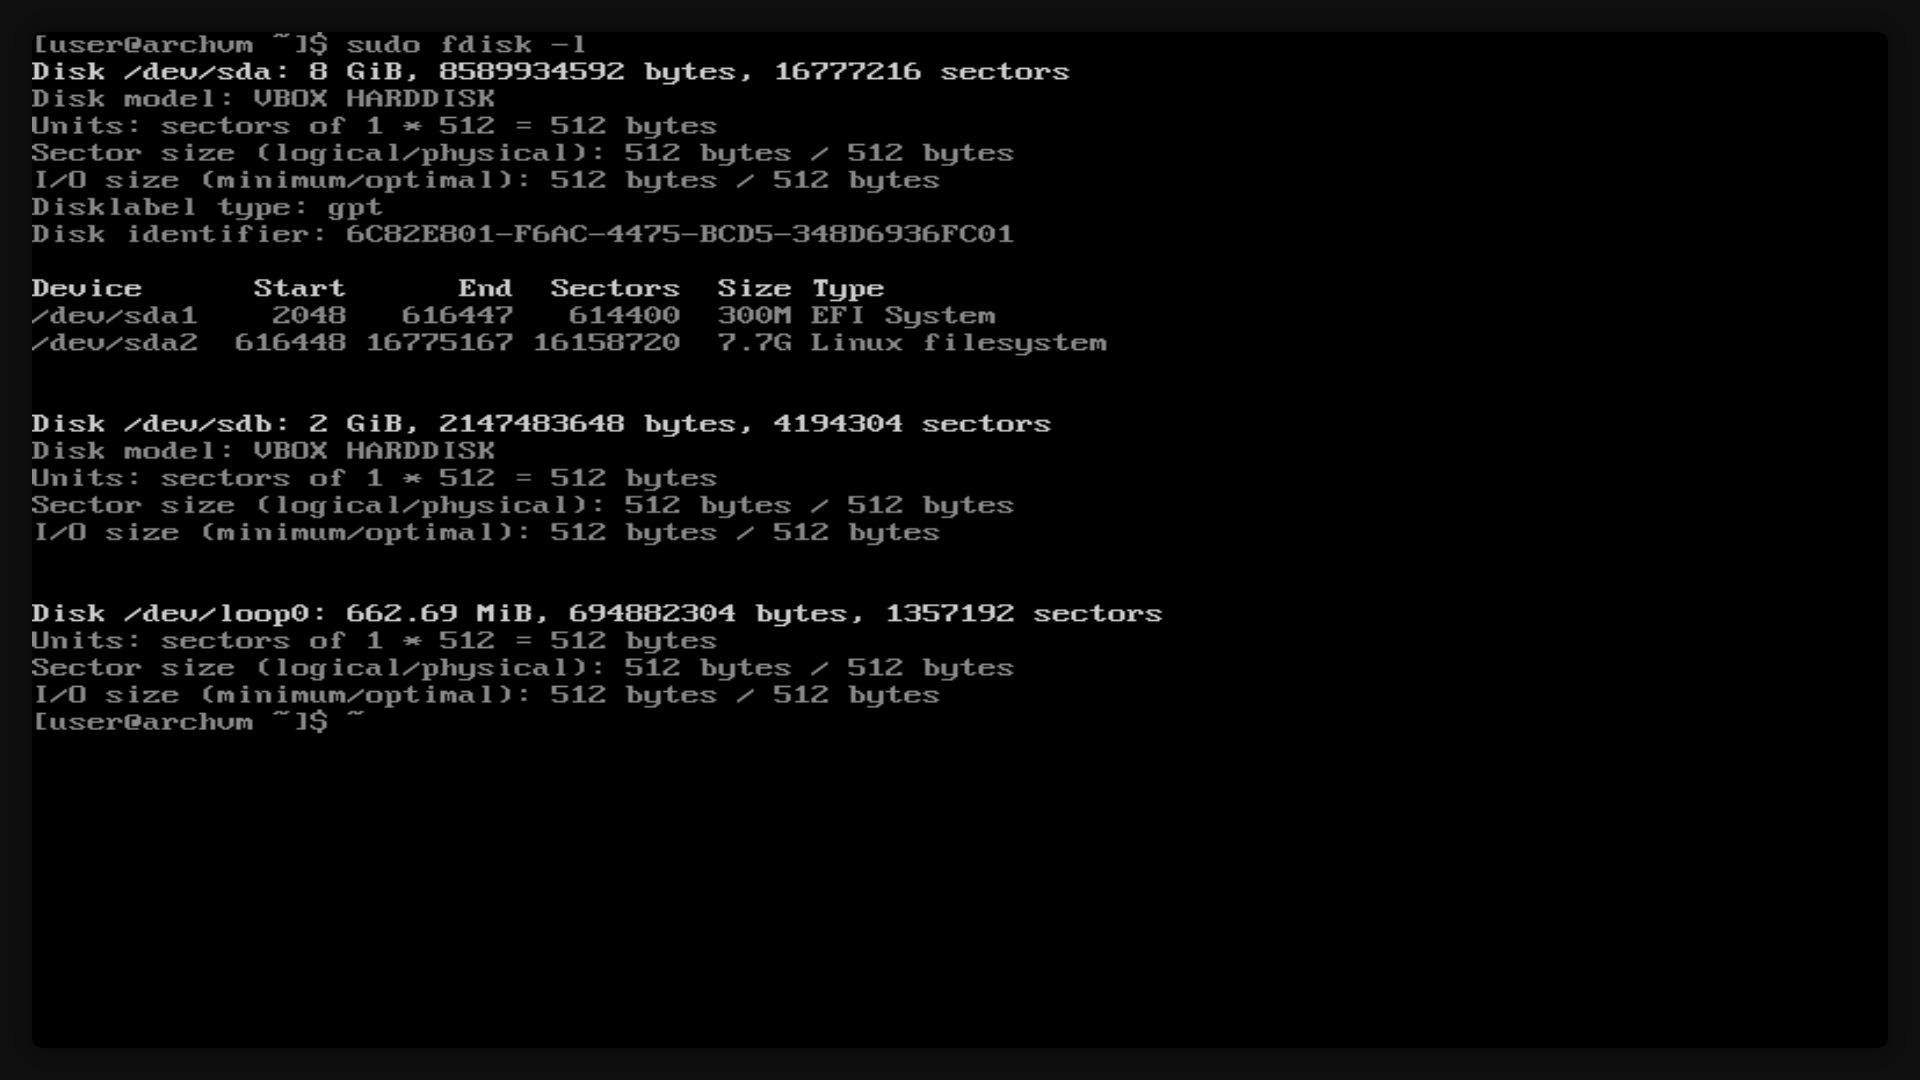
\includegraphics[width=\textwidth,clip=true]{img/2.png}
			\caption{Выводим все блочные устройства, подключенные к виртуальной
			машине. Наш новый виртуальный жесткий диск определился как устройство
			/dev/sdb}
		\end{figure}

	\section{Создание таблицы разделов MBR и дискового тома}
		\begin{figure}[H]
			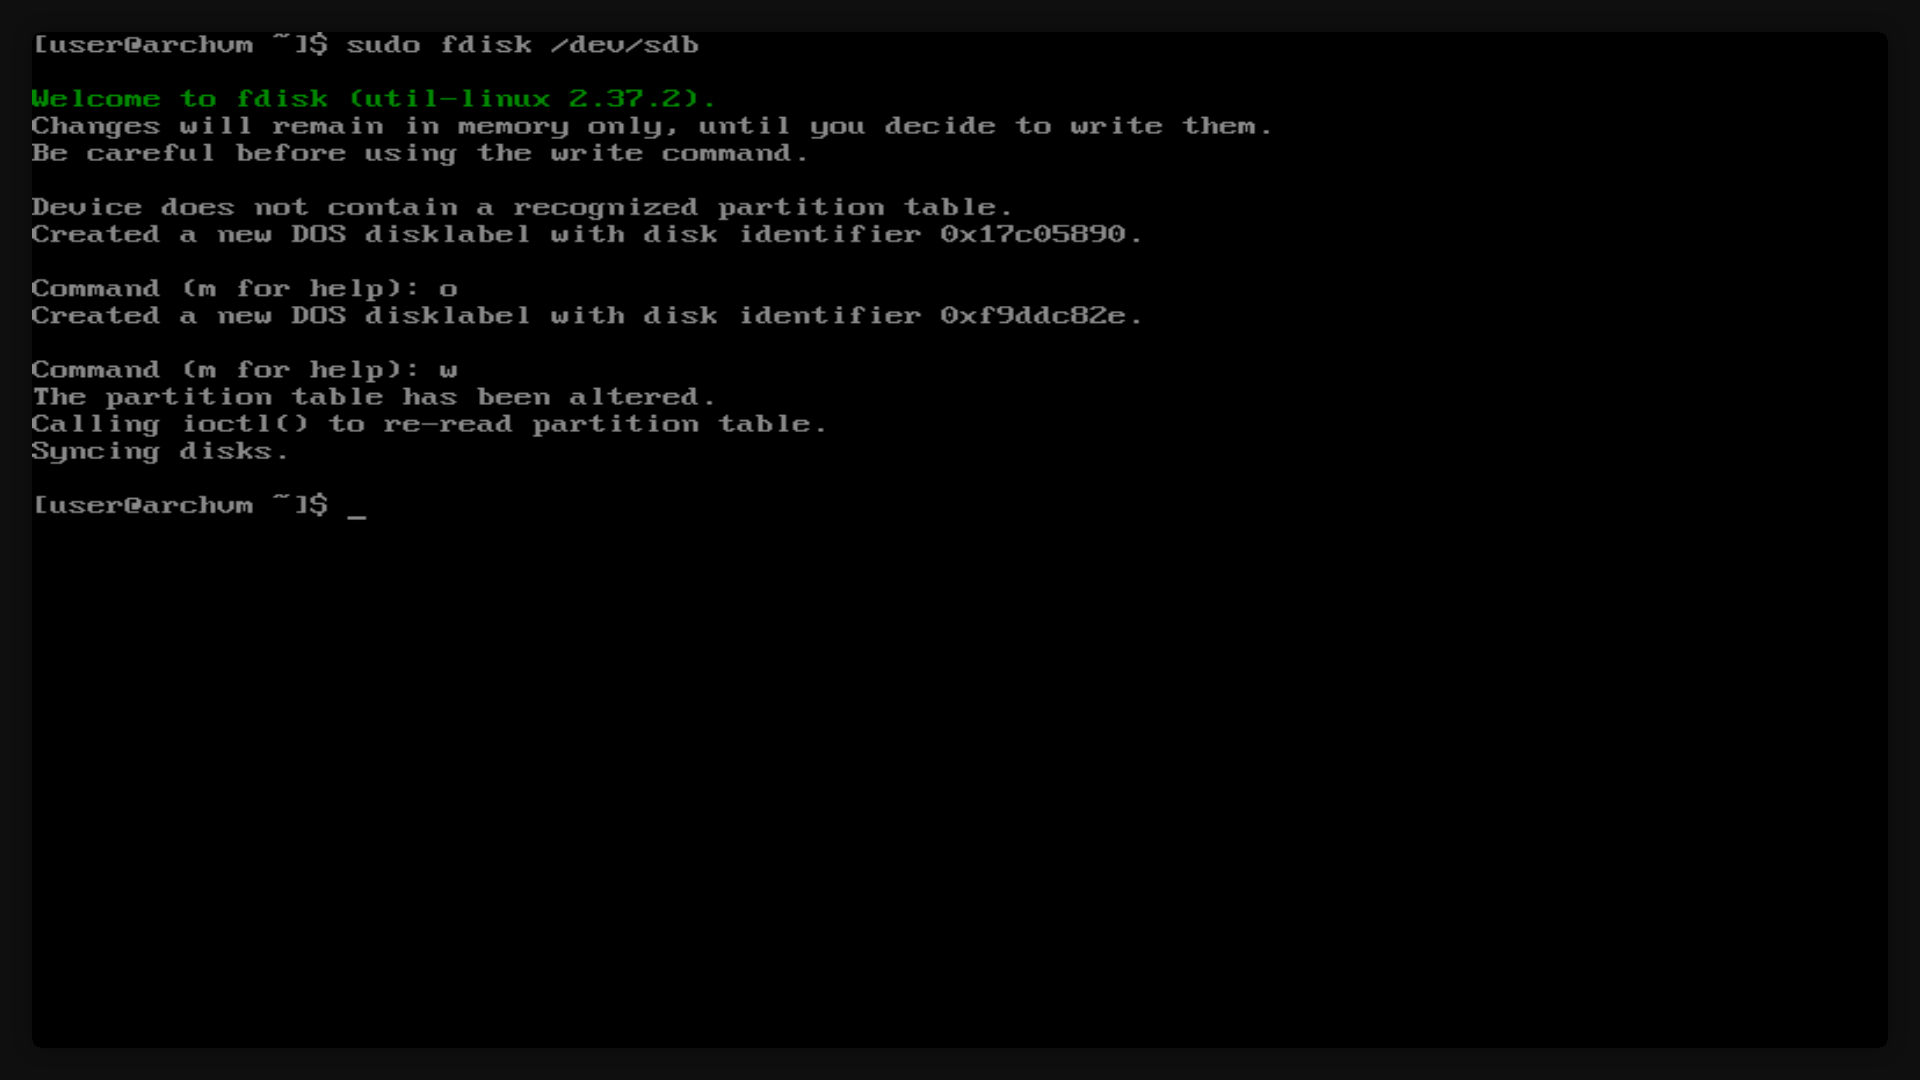
\includegraphics[width=\textwidth,clip=true]{img/3.png}
			\caption{Создаем пустую таблицу разделов MBR}
		\end{figure}

		\begin{figure}[H]
			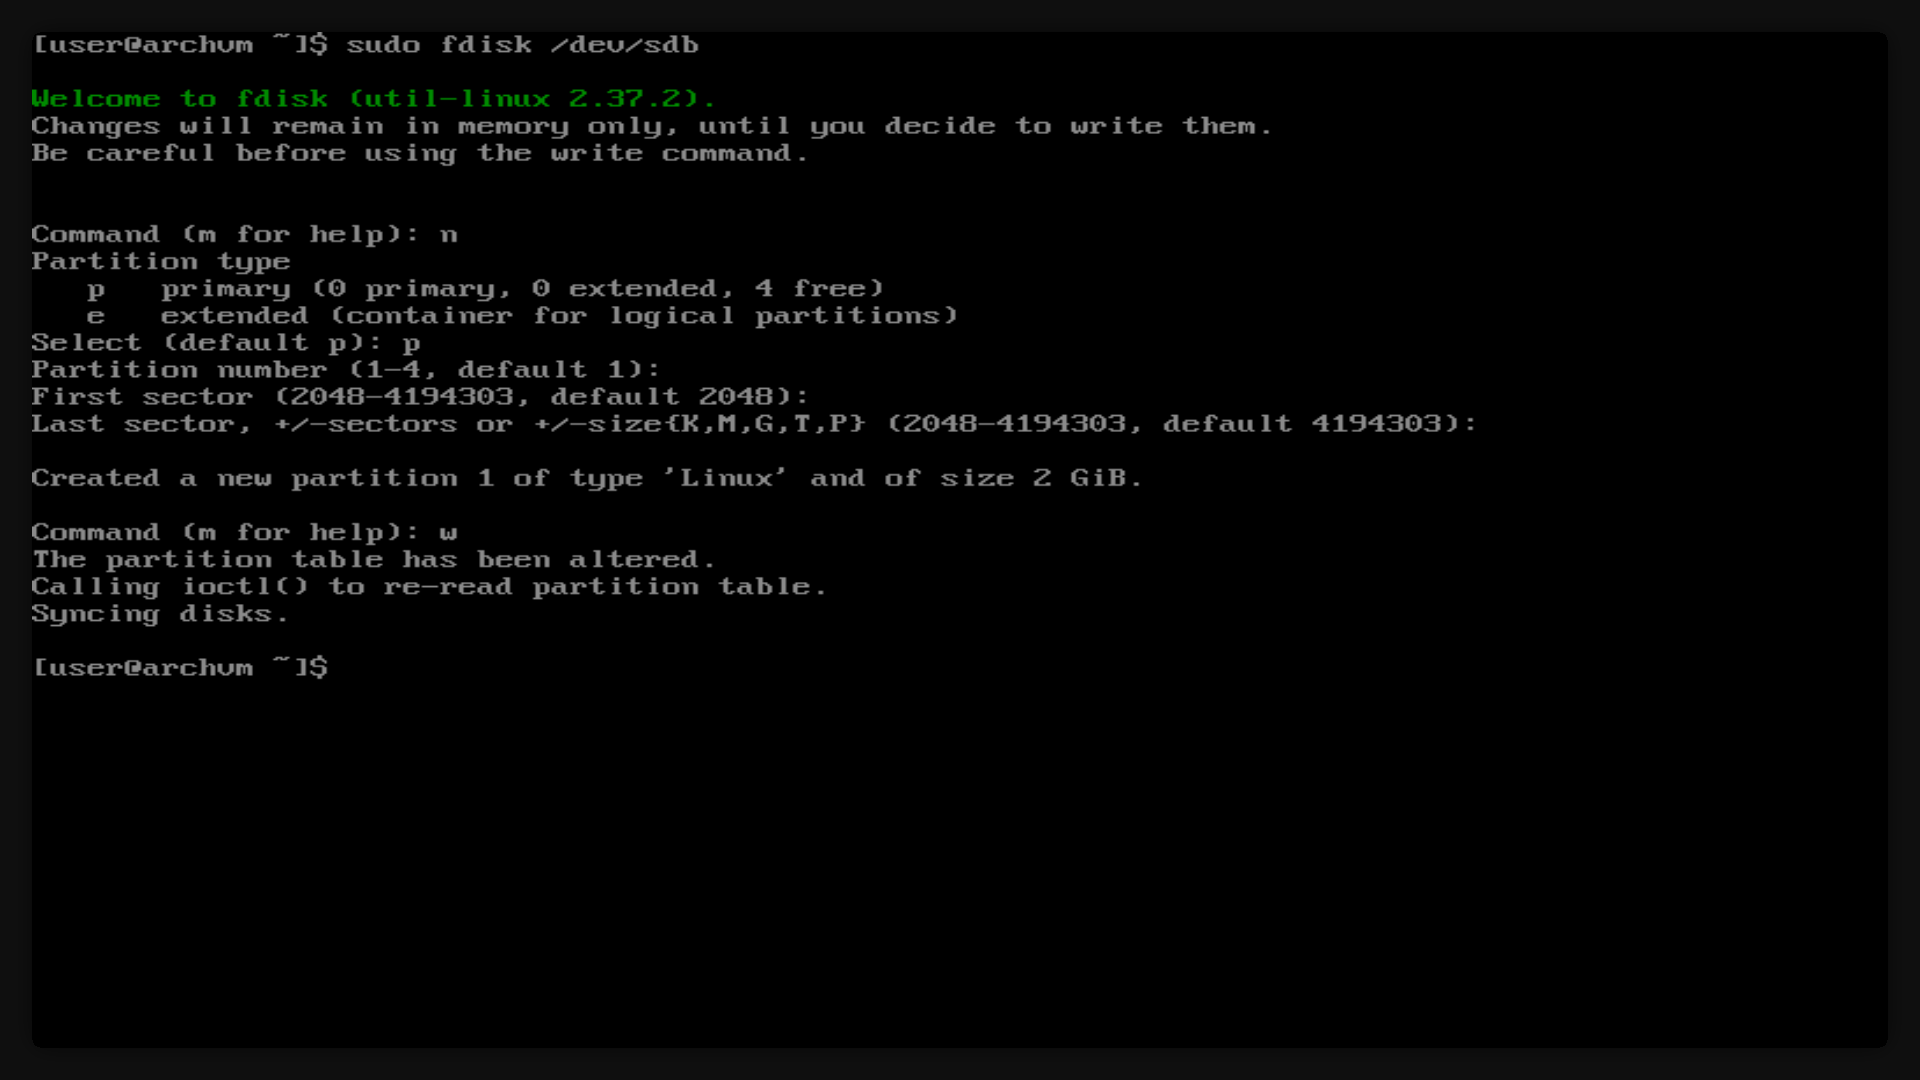
\includegraphics[width=\textwidth,clip=true]{img/4.png}
			\caption{Создаем новый раздел}
		\end{figure}

		\begin{figure}[H]
			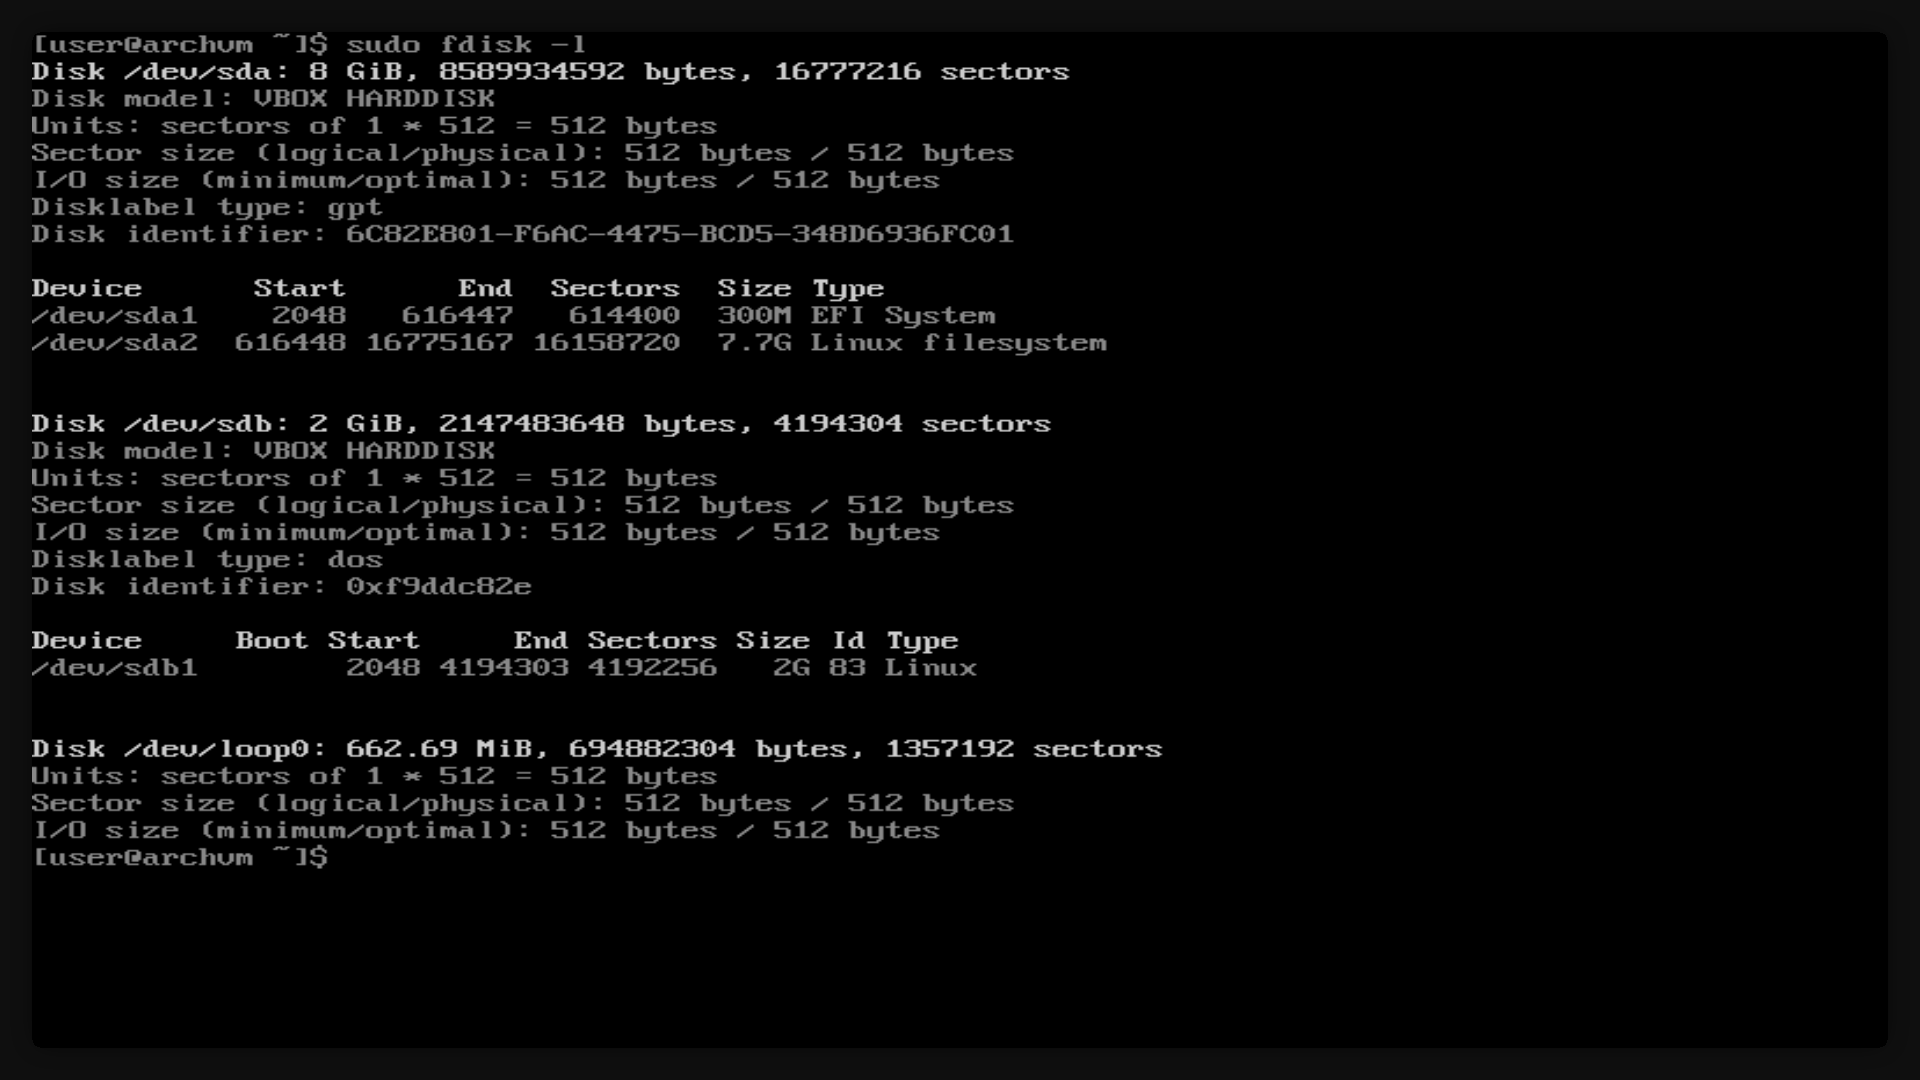
\includegraphics[width=\textwidth,clip=true]{img/5.png}
			\caption{Проверяем результат выполнения манипуляций с блочным устройством}
		\end{figure}

	\section{Форматирование тома и его монтирование}
		\begin{figure}[H]
			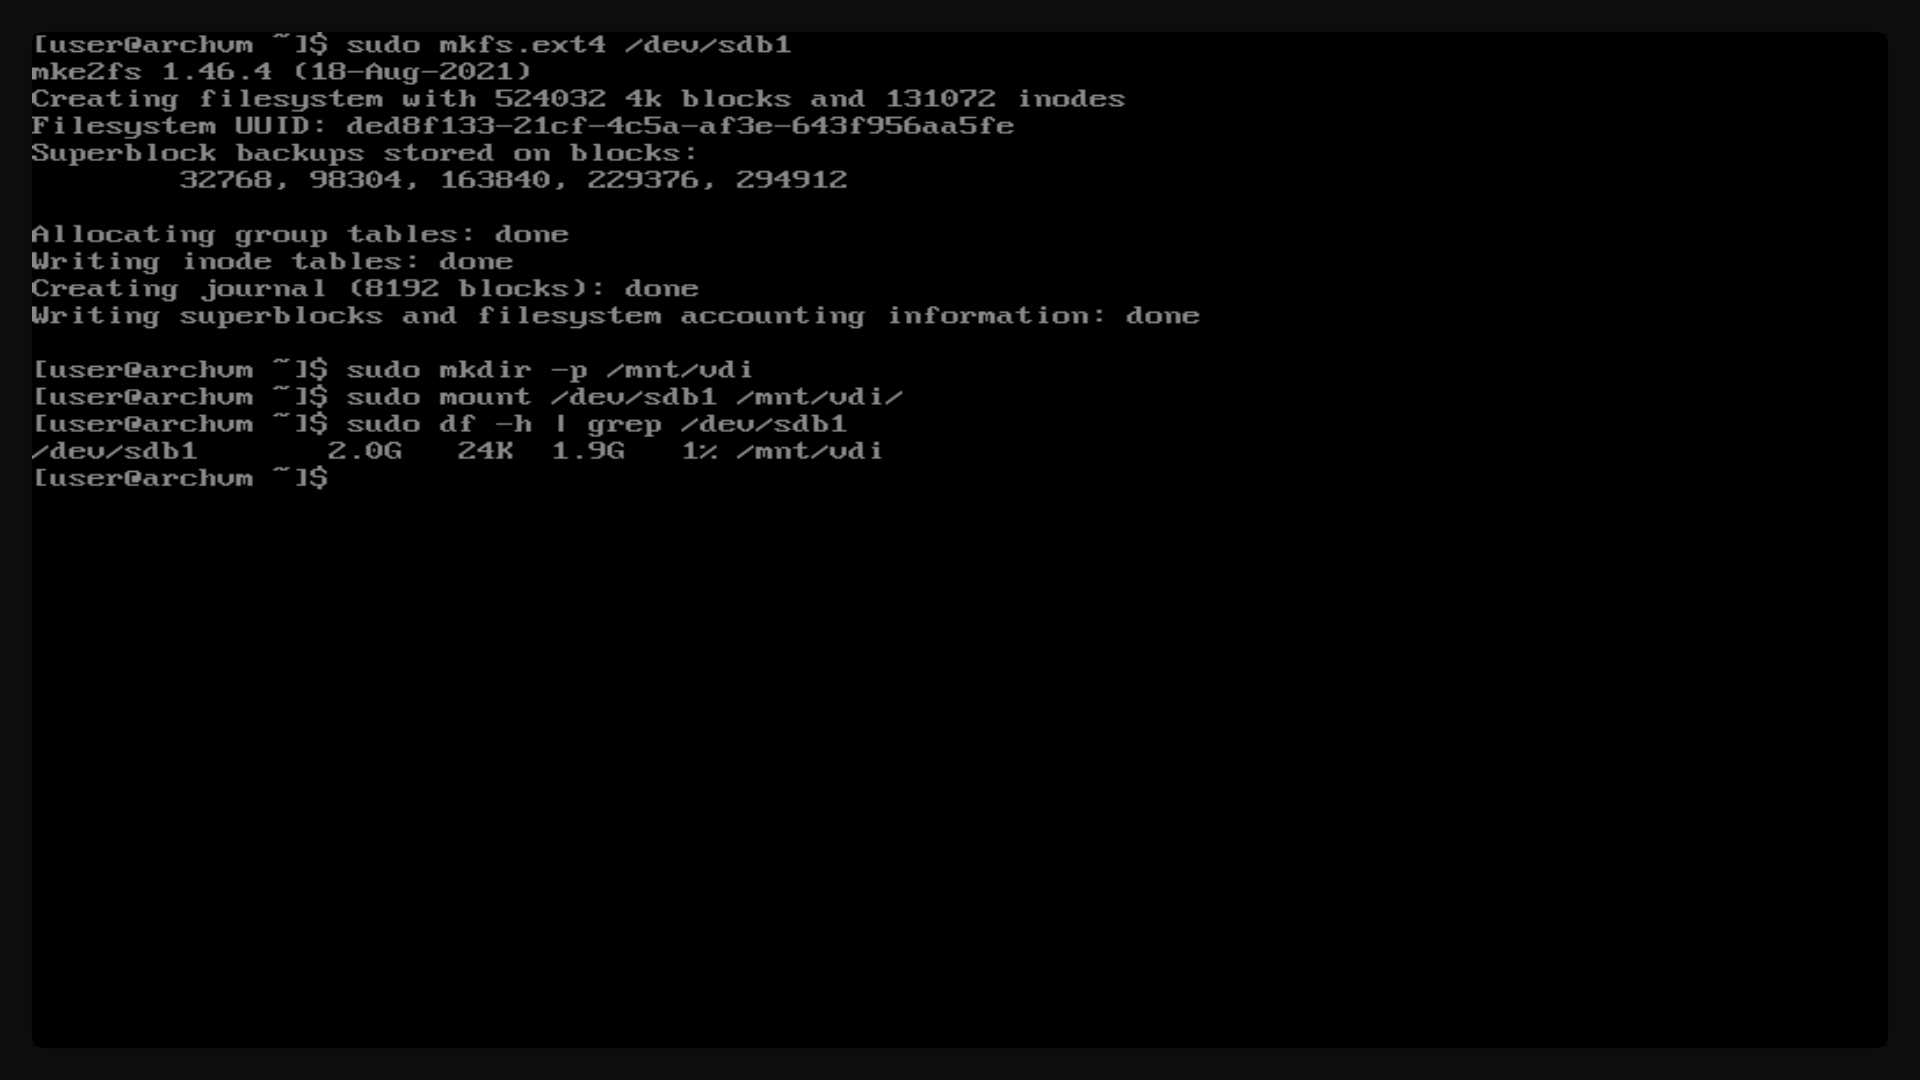
\includegraphics[width=\textwidth,clip=true]{img/6.png}
			\caption{Создаем файловую систему ext4 на разделе и монтируем его в
			директории /mnt/vdi}
		\end{figure}
\end{document}
